%%%%%%%%%%%%%%%%%%%%%%%%%%%%%%%%%%%%%%%%%%%%%%%%%%%%%%%%%%%%%%%%%%%%%%%%%%%%%%%%%%%%%%%%%%
\section{Results and Discussion}


\subsection{Gradient decent methods}

\subsection{Neural Network}

\subsection{Classification}


%  ____            _         _ 
% |  _ \ __ _ _ __| |_    __| |
% | |_) / _` | '__| __|  / _` |
% |  __/ (_| | |  | |_  | (_| |
% |_|   \__,_|_|   \__|  \__,_|
%                              

%%%%%%%%%%%%%%% Run 1 %%%%%%%%%%%%%%%
% Line plot with varying number of mini-batches

In figure \ref{fig:d_line_batch_size} the Accuracy score is plotted for
different number of mini-batches. We observe that the convergence rate
increases with increasing number of mini-batches. This trend is expected. The
total amount of iterations/training is higher for a larger number for
mini batches. Another reason is that we are less likely to get stuck in global
minima, since the multiple different samples is used to calculate gradient of the
cost function. We also observe that the accuracy score tend to increase both
for the training and test data with increasing number of mini-batches.
We chose 20 number of mini-batches as our best value in the next. However, 15
number of mini-batches seems to give similar performance.    


\begin{figure}[H]
    \centering
    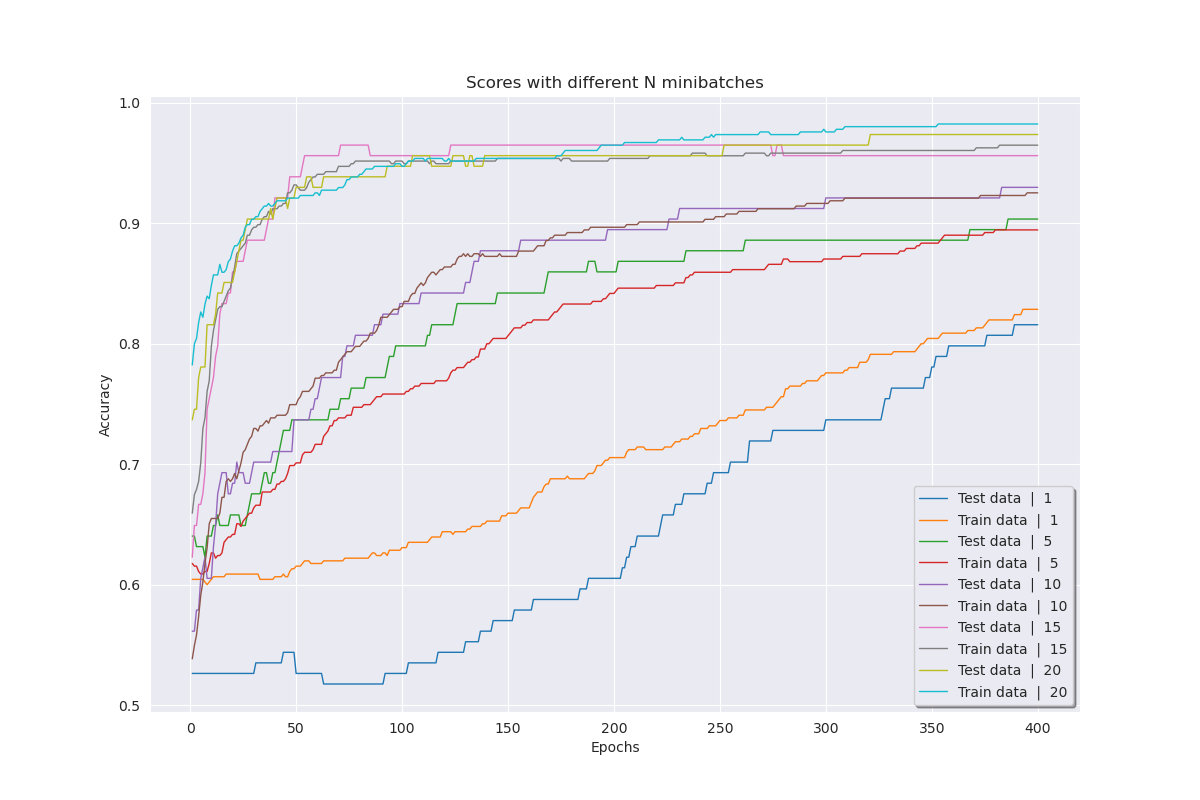
\includegraphics[width=0.8\textwidth]{Figures/PartD/d_line_batch_size.png}
    \caption{Accuracy score for train and test data plottet with respect to epochs for Run 1 (see table
    \ref{tab:runs_classification_cancer}). The number on the labels correspond
to number of mini-batches.}  
    \label{fig:d_line_batch_size} 
\end{figure}


%%%%%%%%%%%%%%% Run 2 %%%%%%%%%%%%%%%

In figure % XXX: ref

In figure \ref{fig:d_heatmap_train_eta_vs_lambda} and
\ref{fig:d_heatmap_train_eta_vs_lambda} is accuracy score for run 2 plotted for
different values of regularization parameter and learning rate for the training
and test data respectively. For our test data the best Accuracy of 0.9825 was
gotten with $\lambda = 10^{-4}$, $\eta = 0.1$ and $\lambda = 0.01$, $\eta =
0.01$. Generally we observe that the accuracy tend to increase with increasing
learning rate. This make sense since the model is learning faster. High
learning rates often leads exploding loss scores. This is not observed in this
case. By choosing the largest learning rate, we can maximize the accuracy and
minimize CPU cycles. 

We observe an increasing trend in accuracy with respect to increasing $\lambda $
values (Lambda in figure). This is more significant for the smaller values
of learning rate. To further study this trend we plotted the accuracy score
for different $\lambda $ values with respect to epochs in figure
\ref{fig:_d_line_different_lambdas}. We clearly see in increased convergence
rate for higher values of lambda. Moreover, the accuracy both for the train and
test data is higher for larger values of $\lambda $. For further fine-tuning of
parameters we will set $\lambda = 0$, to better observe how the different
parameters affect the score with respect to epochs. 


% FIXME: fix figures, 

\begin{figure}[H]
    \centering
    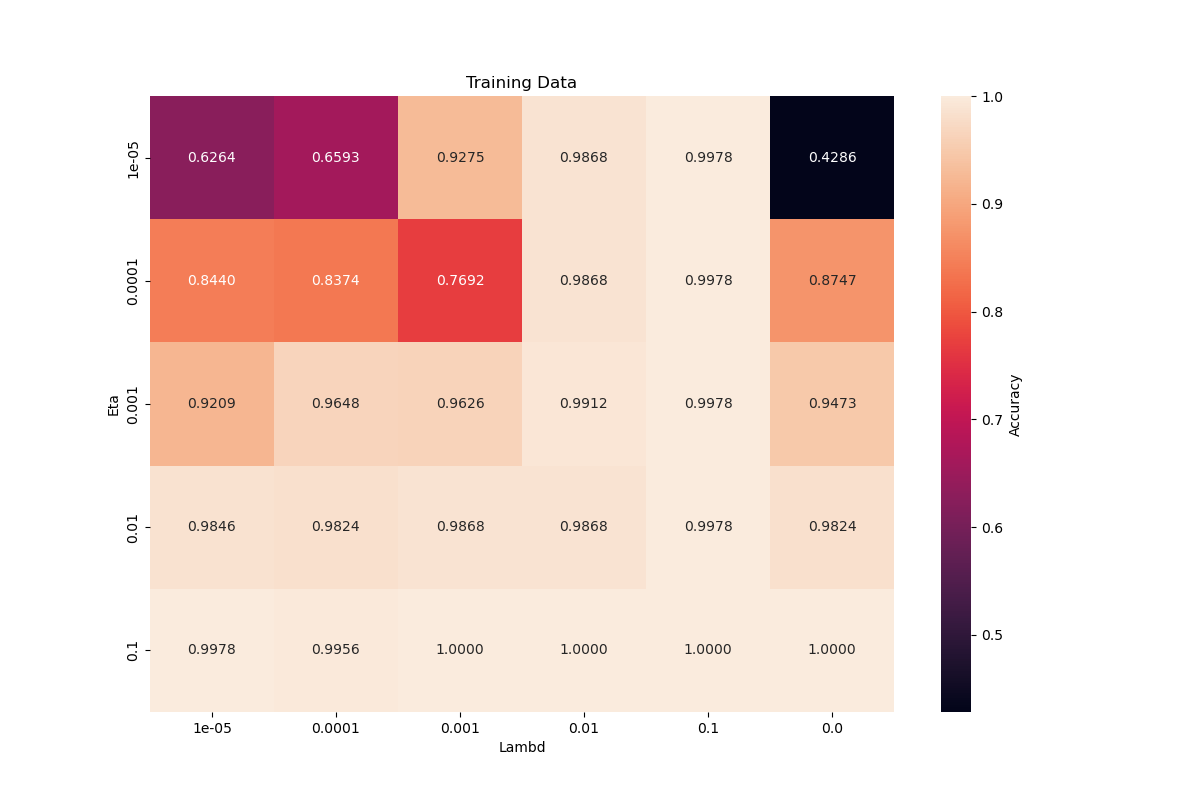
\includegraphics[width=\textwidth]{Figures/PartD/d_heatmap_train_eta_vs_lambda}
    \caption{Heatmap of accuracy score for training dta after 200 epochs with
    respect to different learning rates (Eta) and differn L2-regularzation
    parameters (Lambd).   Spesific parameters used in run 2 is listed in table
\ref{tab:runs_classification_cancer}   }  
    \label{fig:d_heatmap_train_eta_vs_lambda}  
\end{figure}

\begin{figure}[H]
    \centering
    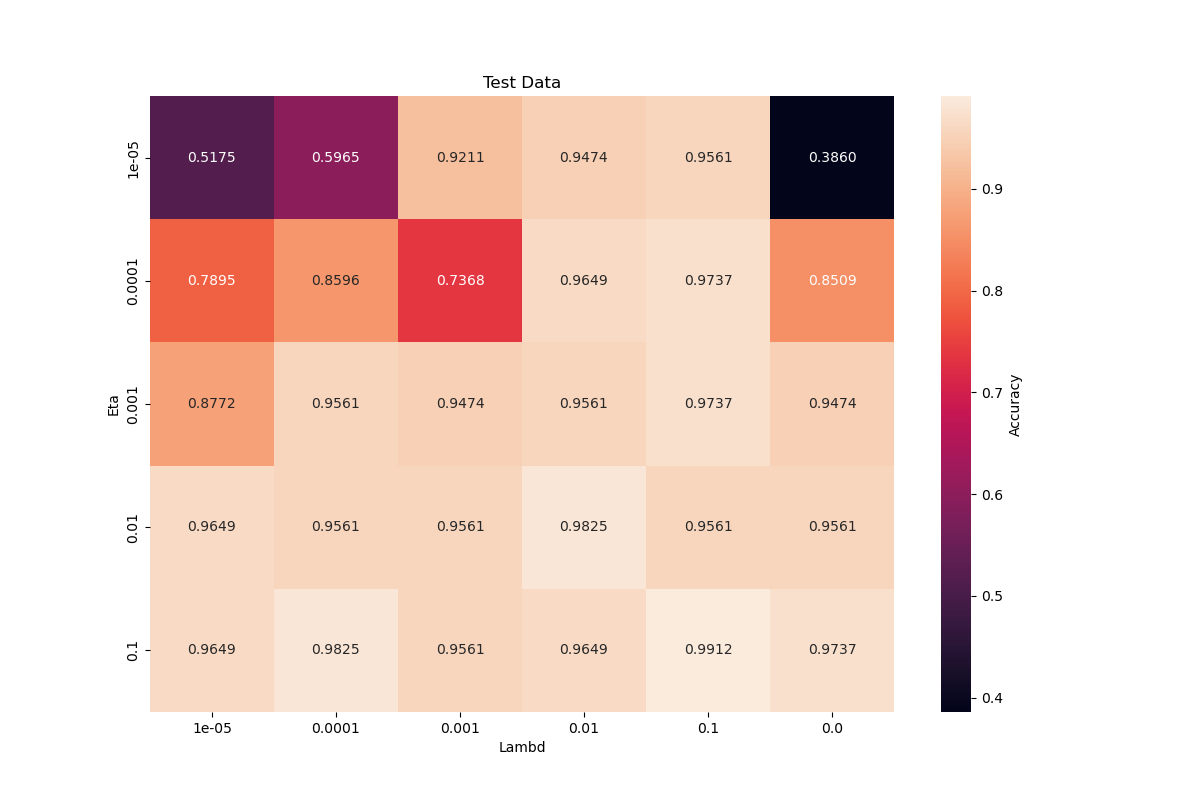
\includegraphics[width=\textwidth]{Figures/PartD/d_heatmap_test_eta_vs_lambda}
    \caption{Heatmap of accuracy score for test dta after 200 epochs with
    respect to different learning rates (Eta) and differn L2-regularization
    parameters (Lambda). Specific parameters used in run 2 is listed in table
    \ref{tab:runs_classification_cancer}       }  
    \label{fig:d_heatmap_test_eta_vs_lambda}  
\end{figure}


            
\begin{figure}[H]
    \centering
    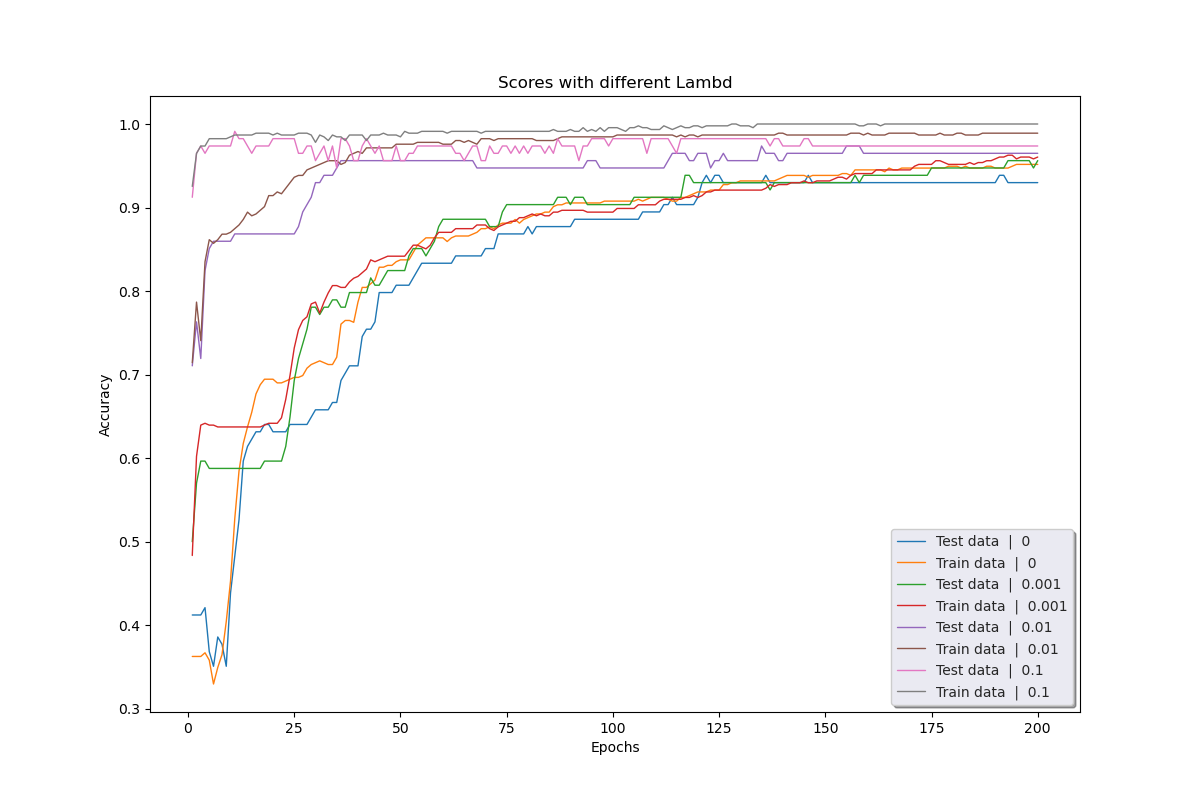
\includegraphics[width=0.8\textwidth]{Figures/PartD/_d_line_different_lambdas.png}
    \caption{Plot of accuracy score for training and test data with respect to
    epochs. Each line correspond to different values of $\lambda $ as indicated
by the number in the legend. A learning rate of 0.001 was used.}  
\label{fig:_d_line_different_lambdas} 
\end{figure}










